\section{Project Scope}

From the literature survey and talking with industry, experts author found many issues they can address when developing the system, but some of those problems like interpretability on autoencoder \citep{ribeiro2016should} are hard to solve by someone at a level of an undergraduate. As this project is done by one developer in less than one year, it won't be possible to create a fully functional monitoring platform like Datadog or New Relic. The focus of this project is to see if the author can develop a single model that can monitor all kinds of services after transfer learning with few examples. \\


\subsection{In-scope} \label{sec:in-scope}
Following are the main focuses of this project
\begin{itemize}[noitemsep,nolistsep] 
    \item Evaluation Framework
    \begin{itemize}[noitemsep,nolistsep] 
        \item Ability to create service mesh out using Kubernetes native resources.
        \item Each service has the ability to simulator predefined error types.
        \item Service mesh can be made up of services written in different programming languages and  frameworks.
        \item Built-in method to run stress tests.
    \end{itemize}
    \item Monitoring System
    \begin{itemize}[noitemsep,nolistsep]
        \item Low overhead data collection pipeline to collect service telemetry.
        \item Reliability system which generate fewer false positives so it won't overwhelm the operators and false negatives will be caught by the main monitoring system.
        \item Optimized models to have fairly small memory footprint and a CPU overhead.
        \item Well generalized model which will be able to deploy with completely new services and it will learn to adapt the new system.
    \end{itemize}
\end{itemize}


\subsection{Out-scope} \label{sec:out-scope}
Follow will not be covered during this project
\begin{itemize}[noitemsep,nolistsep] 
    \item Evaluation Framework
    \begin{itemize}[noitemsep,nolistsep] 
        \item Support for every major language and framework.
        \item Working outside of Kubernetes eco-system.
    \end{itemize}
    \item Monitoring System
    \begin{itemize}[noitemsep,nolistsep] 
        \item Interpretability - Describing a behavior of autoencoder is a difficult task that won't be covered during the project.
        \item System won't be trained against data from a real production system due to the lack of public datasets.
        \item System won't have very high accuracy, as this will be the first line of defense this will try to avoid false positives to prevent adding more noise to alerting systems.
        \item Automatically identify system topology.
        \item This will not be a drop-in replacement for existing monitoring systems, rather this will work with existing monitoring systems to reduce the \ac{mttr}.
    \end{itemize}
\end{itemize}

\subsection{Prototype Feature Diagram}
\begin{figure}[H]
    \centering
    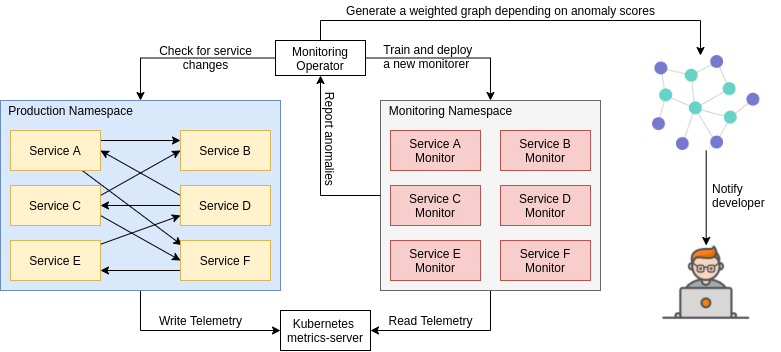
\includegraphics[width=16cm]{assets/introduction/High-level-system-diagram.png}
    \caption{Prototype feature diagram (self composed)}
    \label{fig:high-level-diagram}
\end{figure}